\chapter{Segmentation}

% 3D surface reconstruction (ultrasound)

Thresholding: Based on intensity (simple, but ultrasound intensities can vary a lot).

Region Growing: Start from seed points inside the face region and expand.

Machine Learning / Deep Learning: Modern approaches use CNNs or U-Nets to segment anatomical structures directly in 3D.

Identifying specific regions such as tumors, organs, or vessels.

Can be done via thresholding, region growing, watershed, or deep learning–based methods (e.g., U-Net).

watershed segmentation

\section{U-Net segmentation}

\href{https://github.com/byrkbrk/unet-implementation?tab=readme-ov-file}{unet-implementation}

\begin{center}
  \href{https://github.com/vicente-gonzalez-ruiz/medical_imaging/blob/main/notebooks/unet_cell_data.ipynb}{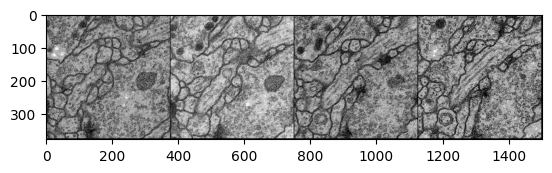
\includegraphics[width=12cm]{unet_cell_data}}
  \href{https://github.com/vicente-gonzalez-ruiz/medical_imaging/blob/main/notebooks/unet_cell_data.ipynb}{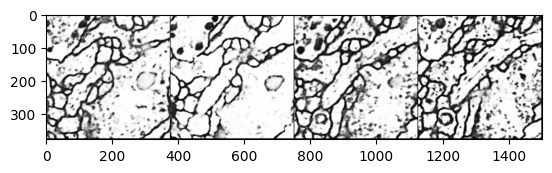
\includegraphics[width=12cm]{unet_cell_data_result}}
\end{center}

